\section{Analyse et Conception du Project}
\subsection{Analyse du besoin}
\begin{frame}{Analyse du besoin}
    \begin{figure}[htpb]
        \centering
        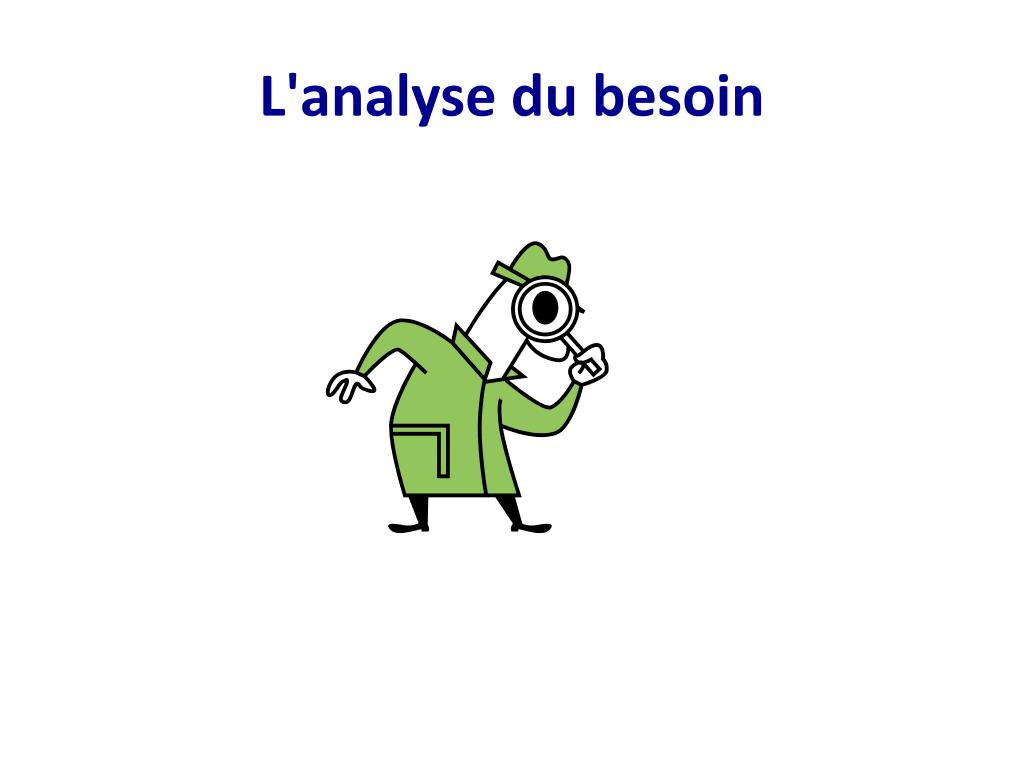
\includegraphics[height=5cm]{assets/images/analyse-besoin.jpg}
    \end{figure}

\end{frame}

\subsection{Digramme cas d'utilisation}
\begin{frame}{Digramme cas d'utilisation}
    \begin{figure}[htpb]
        \centering
        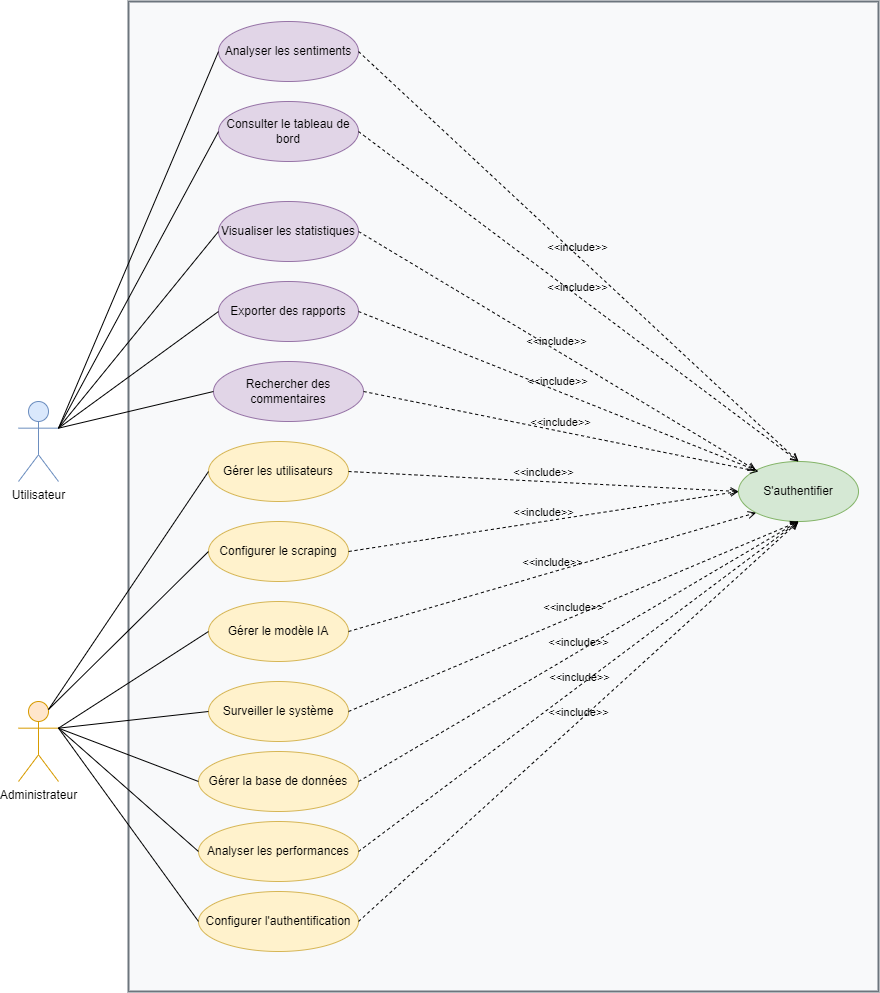
\includegraphics[height=6cm]{assets/images/usecase.png}
    \end{figure}
\end{frame}


\subsection{Architecture microsevice}

\begin{frame}{Architecture microservice}
    \begin{figure}[htpb]
        \centering
        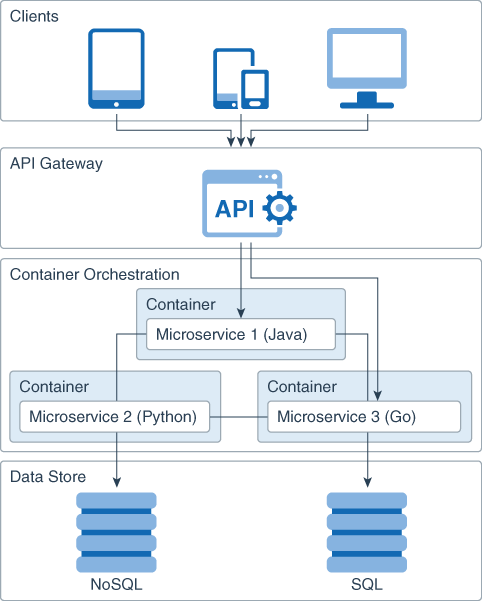
\includegraphics[height=6cm]{assets/images/microservice_architecture_presentation.png}
    \end{figure}
\end{frame}


\begin{frame}{Architectures prévues}
    \begin{figure}[htpb]
        \centering
        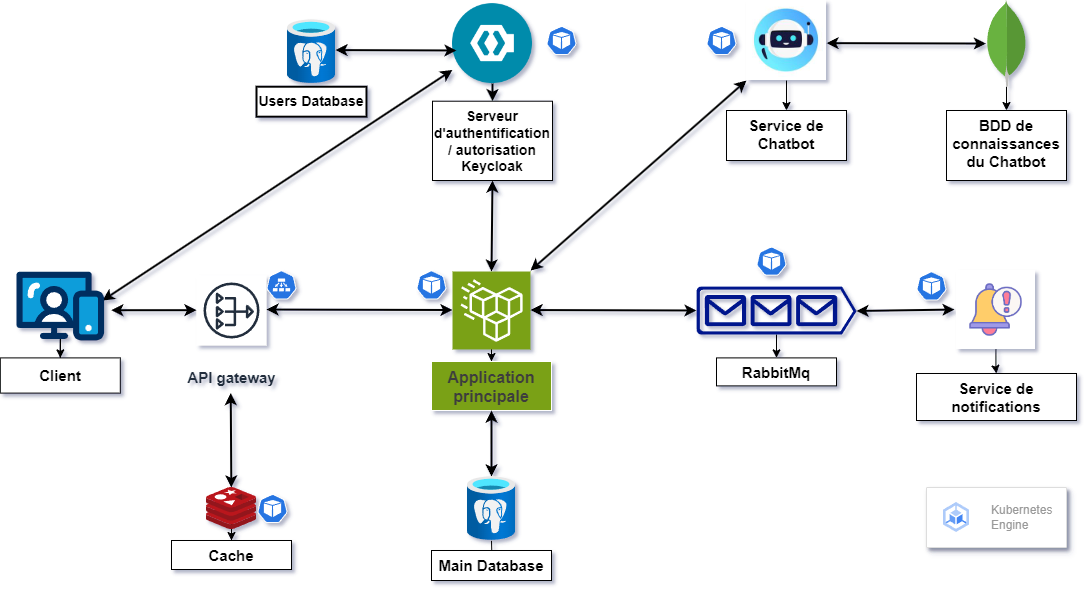
\includegraphics[height=5cm]{assets/images/Code212_architecture.drawio (1).png}
    \end{figure}
\end{frame}

\subsection{Methodology}
\begin{frame}{Methodology}

    \begin{figure}[htpb]
        \centering
        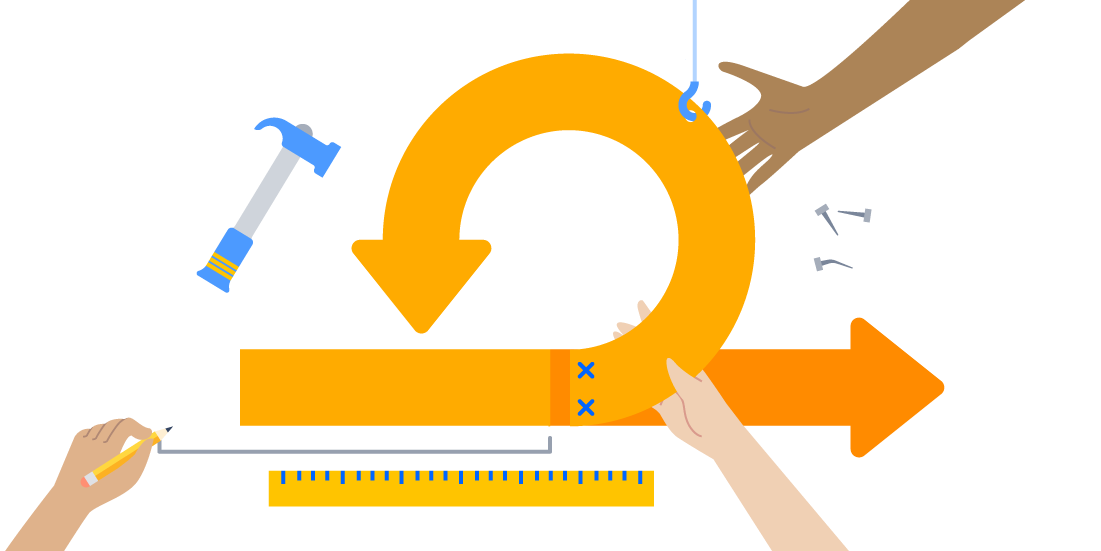
\includegraphics[height=4cm]{assets/images/scrum.png}
    \end{figure}

    Afin de gérer au mieux ce projet, nous avons opté pour la méthode SCRUM et divisé les différents modules en sprints.
\end{frame}


\subsection{Planification}
\begin{frame}{Planification}

    \begin{figure}[htpb]
        \centering
        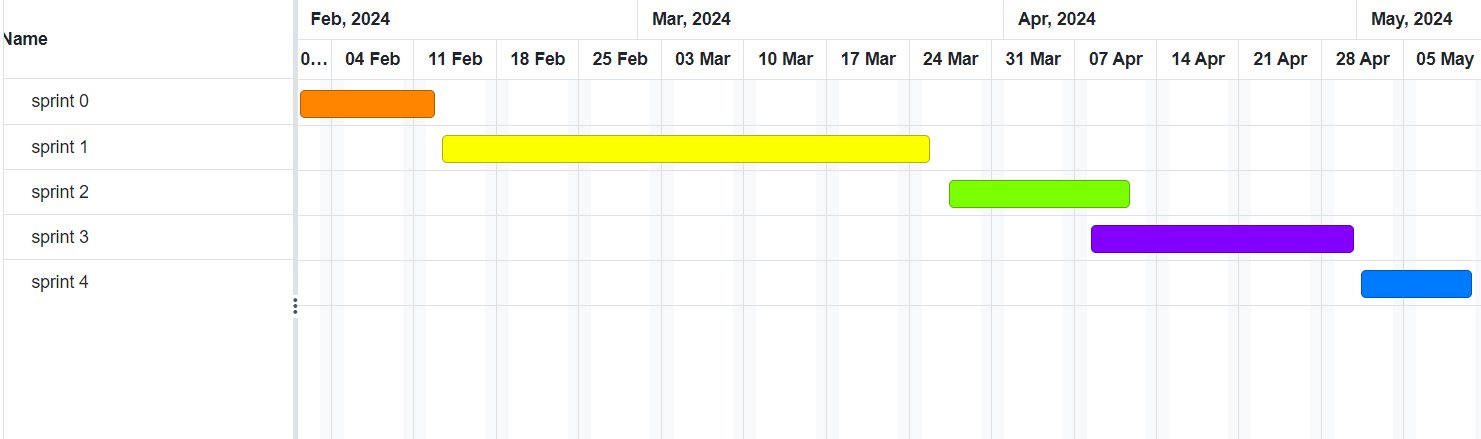
\includegraphics[height=3.5cm]{assets/images/gant-prev.png}
    \end{figure}
\end{frame}




\subsection{Prototype}
\begin{frame}{Prototype}

    \begin{figure}[htpb]
        \centering
        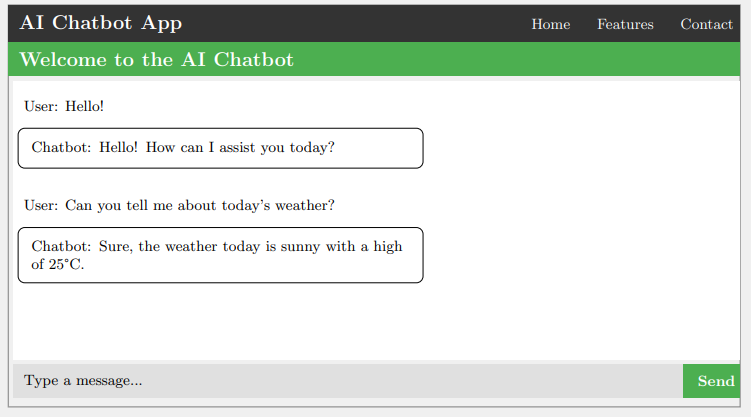
\includegraphics[height=6cm]{assets/images/prototype.png}
    \end{figure}

\end{frame}
